% Options for packages loaded elsewhere
\PassOptionsToPackage{unicode}{hyperref}
\PassOptionsToPackage{hyphens}{url}
\documentclass[
]{article}
\usepackage{xcolor}
\usepackage{amsmath,amssymb}
\setcounter{secnumdepth}{-\maxdimen} % remove section numbering
\usepackage{iftex}
\ifPDFTeX
  \usepackage[T1]{fontenc}
  \usepackage[utf8]{inputenc}
  \usepackage{textcomp} % provide euro and other symbols
\else % if luatex or xetex
  \usepackage{unicode-math} % this also loads fontspec
  \defaultfontfeatures{Scale=MatchLowercase}
  \defaultfontfeatures[\rmfamily]{Ligatures=TeX,Scale=1}
\fi
\usepackage{lmodern}
\ifPDFTeX\else
  % xetex/luatex font selection
\fi
% Use upquote if available, for straight quotes in verbatim environments
\IfFileExists{upquote.sty}{\usepackage{upquote}}{}
\IfFileExists{microtype.sty}{% use microtype if available
  \usepackage[]{microtype}
  \UseMicrotypeSet[protrusion]{basicmath} % disable protrusion for tt fonts
}{}
\makeatletter
\@ifundefined{KOMAClassName}{% if non-KOMA class
  \IfFileExists{parskip.sty}{%
    \usepackage{parskip}
  }{% else
    \setlength{\parindent}{0pt}
    \setlength{\parskip}{6pt plus 2pt minus 1pt}}
}{% if KOMA class
  \KOMAoptions{parskip=half}}
\makeatother
\usepackage{graphicx}
\makeatletter
\newsavebox\pandoc@box
\newcommand*\pandocbounded[1]{% scales image to fit in text height/width
  \sbox\pandoc@box{#1}%
  \Gscale@div\@tempa{\textheight}{\dimexpr\ht\pandoc@box+\dp\pandoc@box\relax}%
  \Gscale@div\@tempb{\linewidth}{\wd\pandoc@box}%
  \ifdim\@tempb\p@<\@tempa\p@\let\@tempa\@tempb\fi% select the smaller of both
  \ifdim\@tempa\p@<\p@\scalebox{\@tempa}{\usebox\pandoc@box}%
  \else\usebox{\pandoc@box}%
  \fi%
}
% Set default figure placement to htbp
\def\fps@figure{htbp}
\makeatother
\ifLuaTeX
  \usepackage{luacolor}
  \usepackage[soul]{lua-ul}
\else
  \usepackage{soul}
\fi
\setlength{\emergencystretch}{3em} % prevent overfull lines
\providecommand{\tightlist}{%
  \setlength{\itemsep}{0pt}\setlength{\parskip}{0pt}}
\usepackage{bookmark}
\IfFileExists{xurl.sty}{\usepackage{xurl}}{} % add URL line breaks if available
\urlstyle{same}
\hypersetup{
  hidelinks,
  pdfcreator={LaTeX via pandoc}}

\author{}
\date{}

\begin{document}

\begin{quote}
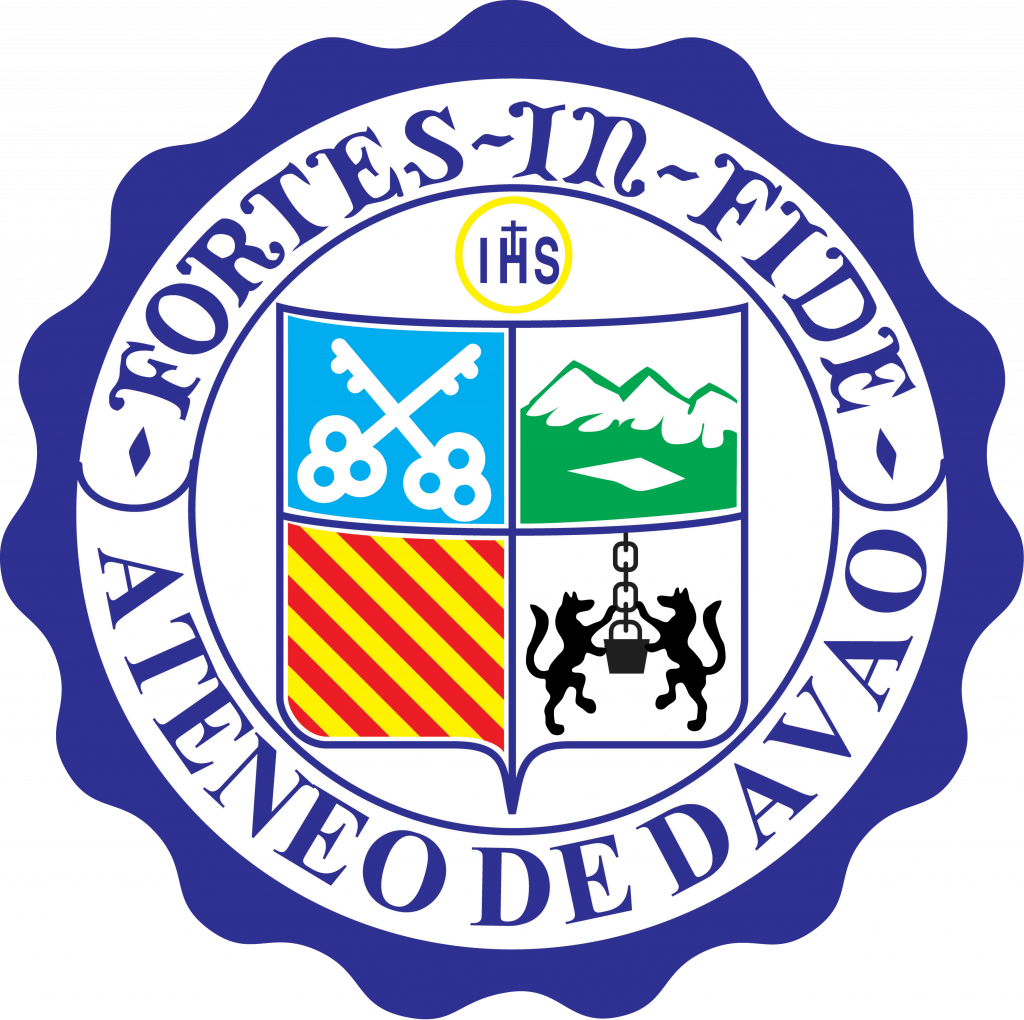
\includegraphics[width=1.84318in,height=1.83333in]{./media/image4.png}
\end{quote}

\textbf{A WEB-BASED DISEASE DATA COLLECTION AND MANAGEMENT SYSTEM FOR
THE ANALYSIS OF GRANULAR AND ANNUAL DATA}

\textbf{Dominic Emmanuel T. Adona, Desiree S. Dagondon, Carlos Manuel S.
Pastores}

\textbf{ATENEO DE DAVAO UNIVERSITY}

\textbf{SCHOOL OF ARTS AND SCIENCES}

\textbf{COMPUTER STUDIES CLUSTER}

\textbf{DAVAO CITY}

\begin{quote}
\textbf{April 2026}
\end{quote}

\textbf{A WEB-BASED DISEASE DATA COLLECTION AND MANAGEMENT SYSTEM FOR
THE ANALYSIS OF GRANULAR AND ANNUAL DATA}

\textbf{A Thesis Presented to the}

\textbf{Faculty of the}

\textbf{Computer Studies Cluster}

\textbf{Ateneo de Davao University}

\textbf{In Partial Fulfillment}

\textbf{of the Requirements for the Degree}

\textbf{Bachelor of Science in Computer Science}

\textbf{By}

\textbf{Dominic Emmanuel T. Adona, Desiree S. Dagondon, Carlos Manuel S.
Pastores}

\textbf{Ateneo de Davao University}

\textbf{School of arts and science}

\textbf{Computer Studies Cluster}

\textbf{April 2026}

\subsubsection{\texorpdfstring{\textbf{Table of
Contents}}{Table of Contents}}\label{table-of-contents}

\textbf{ABSTRACT}
............................................................................................
\textbf{7}

\textbf{CHAPTER 1: INTRODUCTION}

\textbf{1.1 Background of the Study}
........................................................................
\textbf{9}

\textbf{1.2 Statement of the Problem}
......................................................................
\textbf{11}

\textbf{1.2.1 General Problem}
.................................................................................
\textbf{11}

\textbf{1.2.2 Specific Problems}
...............................................................................
\textbf{11}

\textbf{1.3 Objectives of the Study}
.........................................................................
\textbf{12}

\textbf{1.3.1 General Objectives}
.............................................................................
\textbf{12}

\textbf{1.3.2 Specific Objectives}
..............................................................................
\textbf{12}

\textbf{1.4 Significance of the Study}
.......................................................................
\textbf{13}

\textbf{1.5 Scope and Limitations}
...........................................................................
\textbf{14}

\textbf{CHAPTER 2: REVIEW OF RELATED WORKS}

\textbf{2.1 The Philippine Digital Health Landscape and Barangay
Realities} .... \textbf{15}

\textbf{2.2 Technologies for Granular Health Data Management}
......................... \textbf{16}

\textbf{2.2.1 From Manual Registers to Digital Ingestion and Governance}
........ \textbf{16}

\textbf{2.2.2 Relational Database Architectures and Data Normalization}
........... \textbf{16}

\textbf{2.2.3 Local-First Storage and Edge Computing}
........................................ \textbf{17}

\textbf{2.2.4 Python-Based Computational Pipelines for Reporting}
................... \textbf{18}

\textbf{2.2.5 Analysis of Existing Systems and Research Gaps}
......................... \textbf{18}

\textbf{2.2.6 Technical Implementations for Database Security}
.......................... \textbf{19}

\textbf{2.2.7 Data Governance and Lifecycle Protocols}
................................ \textbf{20}

\textbf{2.2.8 Synthesis and Proposed Solution}
.................................................... \textbf{21}

\textbf{2.3 Theoretical Foundations and Frameworks}
......................................... \textbf{22}

\textbf{2.3.1 Theory of Digital Health Resilience (Sustainability)}
....................... \textbf{22}

\textbf{2.3.2 Relational Data Integrity and Normalization Theory}
...................... \textbf{23}

\textbf{2.3.3 Technology Acceptance Model (TAM) and Usability Theory}
........ \textbf{24}

\textbf{2.3.4 Privacy Calculus Theory}
..............................................................
\textbf{25}

\textbf{CHAPTER 3: METHODOLOGY}

\textbf{3.1 Conceptual Framework}
.......................................................................
\textbf{27}

\textbf{3.1.1 Input Stage: Manual Data Ingestion}
................................................ \textbf{28}

\textbf{3.1.2 Process Stage: Local-First Sync and Python Pipelines}
............... \textbf{28}

\textbf{3.1.3 Output Stage: Web Interface and Annual Reports}
........................ \textbf{28}

\textbf{3.2 Operational Framework}
.......................................................................
\textbf{29}

\textbf{3.2.1 Phase I: Data Acquisition and Local Storage}
................................ \textbf{30}

\textbf{3.2.2 Phase II: Synchronization and Compatibility Logic}
...................... \textbf{30}

\textbf{3.2.3 Phase III: Processing and Web Interface}
........................................ \textbf{31}

\textbf{3.2.4 Phase IV: Output Generation and Operational Reporting}
............. \textbf{31}

\textbf{REFERENCES}
....................................................................................
\textbf{33}

\section{\texorpdfstring{\textbf{ABSTRACT}}{ABSTRACT}}\label{abstract}

The management of community-level health intelligence in the Philippines
is increasingly defined by the transition toward high-resolution digital
data architectures. Modern public health informatics frameworks
emphasize the necessity of managing "geographically disaggregated" data
to ensure precision in tracking localized disease trends. Current
literature highlights that while centralized national platforms exist
for regional policy, community-level data management often relies on
manual, paper-based recording or fragmented spreadsheets, leading to
challenges in data normalization and longitudinal reporting. However, a
significant gap remains in the availability of localized digital
infrastructure that can capture case-specific variables at the point of
origin while ensuring data accessibility in varied network environments.
Consequently, this "data siloing" effect limits the capacity for
systematic organization and the automated aggregation of annual health
records. To address these technical limitations, this study proposes a
\textbf{Web-Based Management System} utilizing a \textbf{Relational
Database Architecture} developed with \textbf{Python and SQLite},
incorporating a data sensitivity strategy and \textbf{Role-Based Access
Control (RBAC)} to secure private records. This system implements a
\textbf{"local-first" storage model} to facilitate the collection of
granular disease data and ensure high system availability regardless of
internet connectivity. The proposed framework provides a functional
interface for the digitization of manual community health logs,
establishing a structured digital repository for the retrieval and
analysis of annual barangay health data.

\textbf{Keywords:} \emph{Public Health Informatics, Granular Disease
Data, Relational Database, Local-First Architecture, Python, SQLite,
Data Normalization, Barangay Health Surveillance, Data Privacy,
Role-Based Access Control}

\section{\texorpdfstring{\textbf{CHAPTER 1:
INTRODUCTION}}{CHAPTER 1: INTRODUCTION}}\label{chapter-1-introduction}

\subsubsection{\texorpdfstring{\textbf{1.1 Background of the
Study}}{1.1 Background of the Study}}\label{background-of-the-study}

The management of public health information systems is increasingly
defined by the transition toward high-resolution, decentralized data
architectures. Modern health informatics frameworks emphasize the
necessity of "geographical disaggregation," where data is managed at the
most granular level to ensure precision in health trend analysis
(Glennie et al., 2023). Within the Philippine digital health landscape,
the integration of community-level surveillance into broader national
frameworks depends on the adoption of interoperable digital standards
(Sylim et al., 2022). In highly urbanized centers such as \textbf{Davao
City}, the complexity of monitoring 182 distinct barangays necessitates
a transition from aggregate reports to granular, community-level
monitoring to track active disease cases effectively (\textbf{Otero et
al., 2022}).

From a technical perspective, localized data management often utilizes
traditional recording methods or disparate spreadsheets, which lead to
challenges in data normalization and synchronization. As identified by
Kaboré et al. (2022), the sustainability of digital health in
low-resource settings is frequently compromised by unreliable
infrastructure and technical barriers. Furthermore, the effectiveness of
health dashboards is highly dependent on design components that align
with the specific operational workflows and digital literacy of the
intended end-users (Whitehead et al., 2023; De Mesa et al., 2023).
Consequently, the absence of a unified local database limits the
capacity for longitudinal trend analysis and the systematic organization
of health records over time.

This study implements a Web-Based Management System utilizing a
Relational Database Architecture developed with Python and SQLite. To
ensure high system availability in varied network environments, the
study adopts a "local-first" storage model, a methodology validated for
maintaining data integrity in Philippine rural health settings (Paluyo
et al., 2022). This architecture provides a structured digital
environment for the collection of Granular and Annual Disease Data,
utilizing relational parameters to link individual cases with broader
temporal summaries. By establishing this functional interface, the
system facilitates the transition from manual record-keeping to a
structured digital repository.

\subsubsection{\texorpdfstring{\textbf{1.2 Statement of the
Problem}}{1.2 Statement of the Problem}}\label{statement-of-the-problem}

\textbf{1.2.1 General Problem}

This research aims to develop a Web-Based Management System for the
Collection and Analysis of Granular and Annual Barangay Disease Data to
resolve the technical inefficiencies between manual community-level
record-keeping and high-resolution health monitoring in Barangay Matina
Crossing, Davao City.

\textbf{1.2.2 Specific Problems}

\begin{enumerate}
\def\labelenumi{\arabic{enumi}.}
\item
  How can unstructured granular case attributes (consultation\_date,
  purok\_id, age, gender, disease\_id, and symptoms) across target
  disease vectors (\textbf{Dengue, Leptospirosis, and Tuberculosis}) be
  integrated into a normalized relational schema to maintain data
  integrity and facilitate longitudinal annual reporting?
\item
  How will a local-first storage architecture using an embedded SQLite
  database influence system performance regarding data retrieval query
  latency and record accessibility in an offline-capable environment?
\item
  What is the measurable accuracy rate of the Python-based data pipeline
  in generating automated annual health reports compared to manually
  consolidated historical records?
\item
  What are the quantifiable indicators in a standardized System
  Usability Scale (SUS) test regarding the web interface's effectiveness
  for Barangay Health Workers (BHWs) and Administrators in managing
  localized disease surveillance?
\end{enumerate}

\subsubsection{\texorpdfstring{\textbf{1.3 Objectives of the
Study}}{1.3 Objectives of the Study}}\label{objectives-of-the-study}

\textbf{1.3.1 General Objective}

The main objective of this study is to develop a Web-Based Management
System for the Collection and Analysis of Granular and Annual Barangay
Disease Data to provide a structured digital framework and local-first
architecture for the digitization of community health records and
localized epidemiological surveillance.

\textbf{1.3.2 Specific Objectives}

\begin{enumerate}
\def\labelenumi{\arabic{enumi}.}
\item
  To design and implement a normalized relational database schema that
  maps granular patient-level variables (consultation\_date, purok\_id,
  age, gender, disease\_id, symptoms) for Dengue, Leptospirosis, and
  Tuberculosis into structured annual health summaries.
\item
  To evaluate the execution efficiency of the local-first SQLite
  architecture based on query response times (fetching latency) and
  offline system availability during local network disconnection.
\item
  To quantify the accuracy rate of the Python automated reporting
  pipeline by benchmarking system-aggregated metrics against validated
  manual historical logs from 2023 to 2026.
\item
  To assess the system's interface usability among Barangay Health
  Workers (BHWs) and Administrators using standardized task-completion
  rates and System Usability Scale (SUS) metrics.
\end{enumerate}

\subsubsection{\texorpdfstring{\textbf{1.4 Significance of the
Study}}{1.4 Significance of the Study}}\label{significance-of-the-study}

The primary beneficiaries of this system are \textbf{Local Health Units}
and \textbf{Barangay Health Workers (BHWs)} in Davao City. By providing
a high-resolution tool for localized disease surveillance, the system
mitigates the impact of infrastructure instability and the "digital
divide" prevalent in the Philippines (\textbf{Baticulon et al., 2021}).
Furthermore, city health officials can utilize the aggregated annual
data to optimize resource allocation and public health interventions
based on validated community-level trends (\textbf{Thakur et al.,
2023}), shifting the workflow from reactive reporting to
evidence-grounded monitoring.

This research contributes to the field of \textbf{Public Health
Informatics} by demonstrating a reproducible technical framework for
integrating granular, case-level data with longitudinal annual records
(\textbf{Glennie et al., 2023}). By utilizing a \textbf{local-first
architecture} with SQLite, the study provides a methodology for
maintaining high data availability in varied network environments
(\textbf{Paluyo et al., 2022}; \textbf{Jazaeri et al., 2023}).
Additionally, the use of Python-based pipelines for automated reporting
establishes a model for transforming unstructured manual logs into a
structured relational database capable of high-accuracy temporal trend
analysis (\textbf{Krishnapur et al., 2026}; \textbf{Izonin et al.,
2022}).

This study directly supports \textbf{SDG 3: Good Health and Well-being},
specifically Target 3.D, which aims to strengthen the capacity for early
warning, risk reduction, and management of health risks. By digitizing
community health records, the system improves the accuracy of local
disease tracking.

Furthermore, it aligns with \textbf{SDG 9: Industry, Innovation, and
Infrastructure} by introducing resilient, offline-capable digital
infrastructure to resource-limited settings, and \textbf{SDG 17:
Partnerships for the Goals} by enhancing the availability of
high-quality, timely, and reliable disaggregated data for localized
policy-making.

\subsubsection{\texorpdfstring{\textbf{1.5 Scope and
Limitations}}{1.5 Scope and Limitations}}\label{scope-and-limitations}

The primary scope of this study is the development of a Web-Based
Management System for the structured collection and analysis of Granular
and Annual Barangay Disease Data in Davao City, specifically focused on
\textbf{Dengue, Leptospirosis, and Tuberculosis (TB)}. The system is
built using a Relational Database Architecture implemented with Python
and SQLite to facilitate local-first data storage and retrieval.

In this context, \textbf{Granular Data} refers to individual
consultation records containing seven standardized parameters:
consultation\_date, barangay (defaulted to \emph{Matina Crossing}),
purok\_id, age, gender, disease\_id (Dengue, Leptospirosis, TB), and
symptoms. Conversely, \textbf{Annual Data} refers to the mathematically
aggregated longitudinal summaries covering 2023 to 2026 required for
formal City Health Office (CHO) reporting.

To secure private health records and ensure compliance with the Data
Privacy Act of 2012 (RA 10173), the system enforces strict
de-identification protocols by excluding patient names and contact
details at entry. System governance is enforced through
\textbf{Role-Based Access Control (RBAC),} defining two primary
operational roles:

\begin{itemize}
\item
  \textbf{Barangay Health Workers (BHWs):} Restricted to granular case
  entry, logbook viewing, and local summary monitoring.
\item
  \textbf{Administrators (CHO/Supervisors):} Authorized for full Create,
  Read, Update, and Delete (CRUD) operations on disease logs, as well as
  system user management, role assignments, and account
  activation/blocking via an is\_active status flag.
\end{itemize}

Methodologically, the system is delimited to community-level health data
processing and relies on the accuracy of data inputted by BHWs. The
system functions as a surveillance and storage tool; it excludes
clinical diagnostic capabilities, real-time biological sensors, and
high-level predictive modeling. Offline functionality is restricted to
local data entry, record fetching, and local database operations,
requiring network connectivity only for administrative updates or
centralized synchronization. Finally, the geographic scope is delimited
to Barangay Matina Crossing in Davao City, and the study does not
evaluate patient clinical outcomes or healthcare provider competencies.

\subsection{\texorpdfstring{\textbf{CHAPTER 2: REVIEW OF RELATED
WORKS}}{CHAPTER 2: REVIEW OF RELATED WORKS}}\label{chapter-2-review-of-related-works}

\subsubsection{\texorpdfstring{\textbf{2.1 The Philippine Digital Health
Landscape and Barangay
Realities}}{2.1 The Philippine Digital Health Landscape and Barangay Realities}}\label{the-philippine-digital-health-landscape-and-barangay-realities}

The management of public health information in the Philippines is
characterized by a significant tension between centralized national
strategies and the operational realities of local health units. While
the Philippine National eHealth Strategy advocates for integrated and
interoperable digital systems (\textbf{Sylim et al., 2022}), the
implementation at the community level remains fragmented. \textbf{De
Mesa et al. (2023)} highlight that Barangay Health Workers (BHWs) are
the backbone of this system, yet they operate within a "digital divide"
characterized by infrastructure instability and a lack of specialized
technical tools (\textbf{Baticulon et al., 2021}).

In highly urbanized centers like \textbf{Davao City}, the complexity of
monitoring 182 distinct barangays---ranging from densely populated urban
centers to remote rural zones---creates a "data siloing" effect.
\textbf{Otero et al. (2022)} demonstrate that while pilot studies in
wastewater-based epidemiology provide high-level city data, there is a
critical need for granular, case-specific monitoring at the barangay
level to track active disease trends effectively. Current literature
suggests that until digital tools are grounded in the lived experiences
and connectivity constraints of BHWs (\textbf{Hartigan-Go et al.,
2024}), community-level health intelligence will remain largely manual
and retrospective.

\subsubsection{}\label{section}

\subsubsection{}\label{section-1}

\subsubsection{\texorpdfstring{\textbf{2.2 Technologies for Granular
Health Data
Management}}{2.2 Technologies for Granular Health Data Management}}\label{technologies-for-granular-health-data-management}

\paragraph{\texorpdfstring{\textbf{2.2.1 From Manual Registers to
Digital Ingestion and
Governance}}{2.2.1 From Manual Registers to Digital Ingestion and Governance}}\label{from-manual-registers-to-digital-ingestion-and-governance}

The transition from paper-based logbooks to digital systems is not
merely a change in medium but a shift in governance capability.
\textbf{Thakur et al. (2023)} argue that digitizing manual health
registers enables "meso-level" health officers to make data-driven
decisions rather than relying on delayed aggregate summaries. However,
for digital ingestion to be successful in resource-limited settings,
systems must account for the specific social and professional factors
influencing health professionals (\textbf{Ngusie et al., 2021}). This
necessitates a focus on user-centered design to ensure that digital
transition does not increase the administrative burden on community
workers (\textbf{Whitehead et al., 2023}).

\paragraph{\texorpdfstring{\textbf{2.2.2 Relational Database
Architectures and Data
Normalization}}{2.2.2 Relational Database Architectures and Data Normalization}}\label{relational-database-architectures-and-data-normalization}

The choice of database architecture is a critical technical determinant
of data integrity in health informatics. \textbf{Antas et al. (2022)}
established that Relational Database Management Systems (RDBMS) using
SQL are mathematically more suitable for storing and mining structured
epidemiological datasets compared to NoSQL alternatives.

Furthermore, \textbf{Izonin et al. (2022)} and \textbf{Alderden et al.
(2023)} justify the use of "Data Normalization" as a mechanical
necessity in the medical diagnosis domain. By utilizing relational
parameters to link case-specific variables, a system can ensure that
granular records are synchronized into longitudinal annual summaries
without redundancy or loss of accuracy.

\paragraph{\texorpdfstring{\textbf{2.2.3 Local-First Storage and Edge
Computing}}{2.2.3 Local-First Storage and Edge Computing}}\label{local-first-storage-and-edge-computing}

To address the infrastructure instability documented in the Philippines,
recent research proposes a shift toward "local-first" or "edge"
architectures. The \textbf{"Padayon" model (Paluyo et al., 2022)} serves
as a primary validation of offline-first digital health models in rural
Philippines, proving that data integrity can be maintained without
constant internet connectivity. From a performance perspective,
\textbf{Jazaeri et al. (2023)} demonstrate that processing data at the
"edge"---on the local device rather than a remote server---minimizes
latency and optimizes data classification for IoT and web-based
healthcare solutions. This ensures that BHWs can retrieve and input data
with high speed, regardless of the local network state.

\paragraph{\texorpdfstring{\textbf{2.2.4 Python-Based Computational
Pipelines for
Reporting}}{2.2.4 Python-Based Computational Pipelines for Reporting}}\label{python-based-computational-pipelines-for-reporting}

Modern public health informatics requires more than just storage; it
requires the automated transformation of raw data into intelligence.
\textbf{Krishnapur et al. (2026)} validate the use of Python-based
computational pipelines for the real-time ingestion and dynamic
reporting of public health data.

Such frameworks allow for the creation of reproducible analysis paths,
ensuring that annual reports generated by the system are consistent with
the raw granular inputs. This technical standard supports the transition
from "data collection" to "health monitoring" by providing stakeholders
with automated, high-resolution summaries.

\subsubsection{\texorpdfstring{\textbf{2.2.5 Analysis of Existing
Systems and Research
Gaps}}{2.2.5 Analysis of Existing Systems and Research Gaps}}\label{analysis-of-existing-systems-and-research-gaps}

Despite advancements in health informatics, several critical gaps
persist:

\begin{itemize}
\item
  \textbf{The Resolution Mismatch:} Most national platforms (e.g.,
  iPHOIS) focus on regional or provincial summaries, leaving a void for
  high-resolution, barangay-level granular tracking in cities like
  Davao.
\item
  \textbf{The Connectivity Dependency:} A majority of existing web-based
  management systems follow an "always-online" cloud model, which fails
  to satisfy the resilience requirements of Philippine community health
  settings (\textbf{Kaboré et al., 2022}).
\item
  \textbf{The Normalization Gap:} While digital tools exist for data
  entry, there is a lack of integrated frameworks that automatically
  normalize unstructured manual logs into structured relational
  repositories for annual longitudinal analysis.
\end{itemize}

\textbf{2.2.6 Technical Implementations for Database Security}

Securing localized health data in a Python and SQLite environment
requires a multi-layered defense to build user trust and meet regulatory
standards. The architecture implements four core security controls:

\begin{itemize}
\item
  \textbf{Data Privacy Compliance (RA 10173):} In compliance with the
  Philippine Data Privacy Act of 2012, direct identifiers (names, phone
  numbers, addresses) are excluded from the schema. Consultation logs
  receive auto-generated internal keys (id) to ensure point-of-entry
  de-identification.
\item
  \textbf{Role-Based Access Control (RBAC):} BHW permissions are
  restricted to data entry and local logbook viewing. Administrative
  roles hold full CRUD privileges over disease logs and manage account
  activation using an is\_active status flag. .
\item
  \textbf{Credential Protection (Flask-Bcrypt):} User passwords are
  secured using Flask-Bcrypt key-stretched salted hashing, mitigating
  brute-force attacks while maintaining fast local execution.
\item
  \textbf{At-Rest Encryption:} Local database files (lokalhealth.db) are
  encrypted using SQLCipher with 256-bit AES, while sensitive app keys
  use Python Fernet encryption to protect offline edge deployments
  against hardware theft.
\end{itemize}

\textbf{2.2.7 Data Governance and Lifecycle Protocols}

Adopting a formal governance structure is critical for transforming raw
community inputs into high-integrity health assets. According to
\textbf{Oktaviana R. et al. (2025)}, effective health data governance is
foundational to improving patient safety and establishing clear
accountabilities for data protection, particularly in developing
nations, where research in this domain remains emergent. This study
identifies that addressing issues such as data redundancy and incomplete
records requires a focus on three core domains: data quality management,
metadata management, and data security.

To operationalize these governance domains, the proposed system follows
the \textbf{Data Life Cycle Management (DLCM)} model established by
\textbf{Rahul and Banyal (2020)}. This model maps the data journey
through six distinct phases: creation, storage, usability, sharing,
archiving, and destruction. By implementing this lifecycle under a
secure management system, the project ensures that granular health data
remains accessible for immediate barangay use while being structured for
long-term "archive" and "sharing" in the form of annual CHO reports.

\subsubsection{}\label{section-2}

\subsubsection{\texorpdfstring{\textbf{2.2.8 Synthesis and Proposed
Solution}}{2.2.8 Synthesis and Proposed Solution}}\label{synthesis-and-proposed-solution}

To address these multi-dimensional gaps, this study proposes a Web-Based
Disease Data Collection and Management System designed for the barangay
level. Unlike centralized national platforms, this system focuses on
high-resolution data capture, allowing for the tracking of individual
cases (granular data) that are structured to aggregate into longitudinal
summaries (annual data).

To address the \textbf{Connectivity Dependency}, the study proposes a
\textbf{Local-First Architecture} utilizing \textbf{SQLite}. This design
allows Barangay Health Workers to perform data entry and retrieval tasks
without a constant internet connection, synchronizing with the central
repository when bandwidth is available.

Furthermore, to address the \textbf{Privacy and Security Gap}, the
proposed system implements a multi-layered cryptographic framework. By
utilizing \textbf{SQLCipher} for at-rest database encryption and
\textbf{bcrypt} for credential hashing, the system directly mitigates
the "Perceived Risks" identified in the \textbf{Privacy Calculus
Theory}, thereby increasing the likelihood of user adoption and data
sharing.

Finally, to address the \textbf{Normalization Gap}, the system utilizes
a \textbf{Python-based framework} to map unstructured inputs into a
normalized database schema. This technical approach transforms
fragmented community health logs into a structured digital repository,
providing stakeholders with a grounded tool for localized health
surveillance.

\subsubsection{\texorpdfstring{\textbf{2.3 Theoretical Foundations and
Frameworks}}{2.3 Theoretical Foundations and Frameworks}}\label{theoretical-foundations-and-frameworks}

\paragraph{\texorpdfstring{\textbf{2.3.1 Theory of Digital Health
Resilience
(Sustainability)}}{2.3.1 Theory of Digital Health Resilience (Sustainability)}}\label{theory-of-digital-health-resilience-sustainability}

Grounding the study's architecture, this theory posits that for digital
health interventions to be sustainable in low- and middle-income
countries, they must be resilient to infrastructure failure. As
supported by \textbf{Kaboré et al. (2022)}, this \textbf{justifies} the
implementation of a \textbf{Local-First Architecture}. This framework
ensures that the system functions in a "degraded" network state,
treating synchronization as a background process rather than a
requirement for operation.

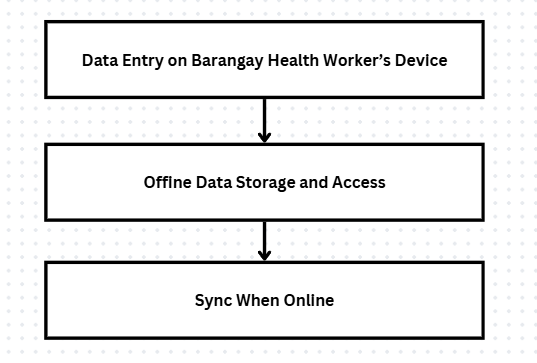
\includegraphics[width=5.59375in,height=3.78125in]{./media/image5.png}

\textbf{Figure 2.3.1. Theory of Digital Health Resilience
(Sustainability)}

\paragraph{\texorpdfstring{\textbf{2.3.2 Relational Data Integrity and
Normalization
Theory}}{2.3.2 Relational Data Integrity and Normalization Theory}}\label{relational-data-integrity-and-normalization-theory}

This theory provides the mathematical basis for the system's data
structure. It suggests that medical data accuracy is directly tied to
the minimization of data redundancy through normalization rules
(\textbf{Izonin et al., 2022}). This justifies the use of a relational
schema in \textbf{SQLite} to link individual disease cases with temporal
annual summaries, ensuring that "Granular" data is technically
compatible with "Annual" reporting requirements.

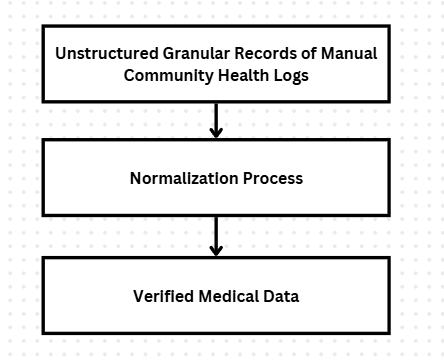
\includegraphics[width=4.625in,height=3.76042in]{./media/image1.png}

\textbf{Figure 2.3.2. Relational Data Integrity and Normalization
Theory}

\paragraph{}\label{section-3}

\paragraph{\texorpdfstring{\textbf{2.3.3 Technology Acceptance Model
(TAM) and Usability
Theory}}{2.3.3 Technology Acceptance Model (TAM) and Usability Theory}}\label{technology-acceptance-model-tam-and-usability-theory}

The final pillar of the framework addresses the human-computer
interaction (HCI) aspect. According to TAM, a system's adoption is
determined by its \textbf{Perceived Ease of Use} and \textbf{Perceived
Usefulness}. This theory, validated for culturally diverse populations
by \textbf{Whitehead et al. (2023)}, justifies the use of standardized
usability metrics to assess how effectively Barangay Health Workers can
manage localized disease surveillance through the system's interface.

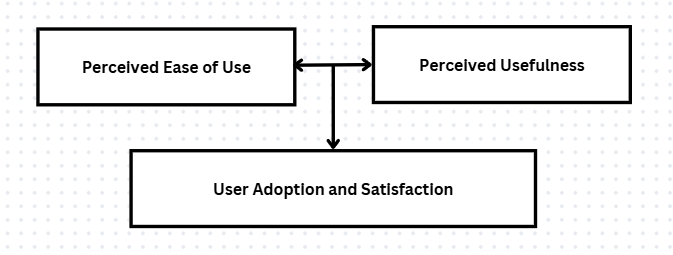
\includegraphics[width=5.61458in,height=2.67708in]{./media/image7.png}

\textbf{Figure 2.3.3 Technology Acceptance Model (TAM) and Usability
Theory}

\subsubsection{\texorpdfstring{\textbf{2.3.4 Privacy Calculus
Theory}}{2.3.4 Privacy Calculus Theory}}\label{privacy-calculus-theory}

This theory provides the psychological and decision-making framework for
data sharing in health tracking systems. As established by \textbf{Li et
al. (2023)}, individuals engage in a "calculus" where they weigh the
\textbf{perceived privacy risks} (e.g., data breaches or hardware theft)
against the \textbf{perceived benefits} of public service utility.

This theory justifies the inclusion of robust security measures such as
\textbf{At-Rest Encryption} and \textbf{Credential Hashing} not just as
technical requirements, but as essential tools to mitigate user risk
perception. By reducing the "potential loss expectations" through
visible security protocols, the system increases the user's intention to
provide the granular data necessary for accurate health monitoring.

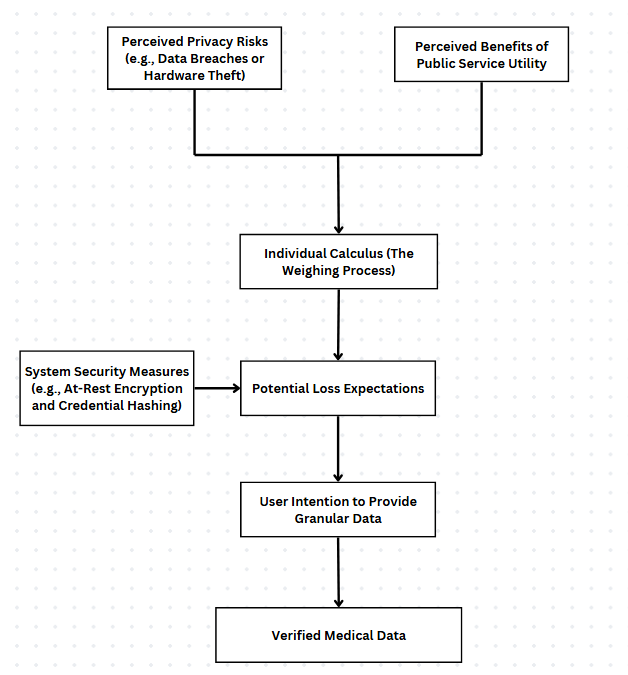
\includegraphics[width=6.62963in,height=7.12898in]{./media/image6.png}

\textbf{Figure 2.3.4 Privacy Calculus Theory}

\subsubsection{}\label{section-4}

\subsubsection{\texorpdfstring{\textbf{CHAPTER 3:
METHODOLOGY}}{CHAPTER 3: METHODOLOGY}}\label{chapter-3-methodology}

\textbf{3.1 Conceptual Framework}

The conceptual framework of this study follows an
\textbf{Input-Process-Output (IPO)} model, illustrating the systematic
transformation of fragmented manual health records into actionable,
structured health intelligence. This framework (see Figure 3.1)
integrates local-first synchronization and automated data pipelines to
provide high-resolution reporting for the barangays of Davao City.

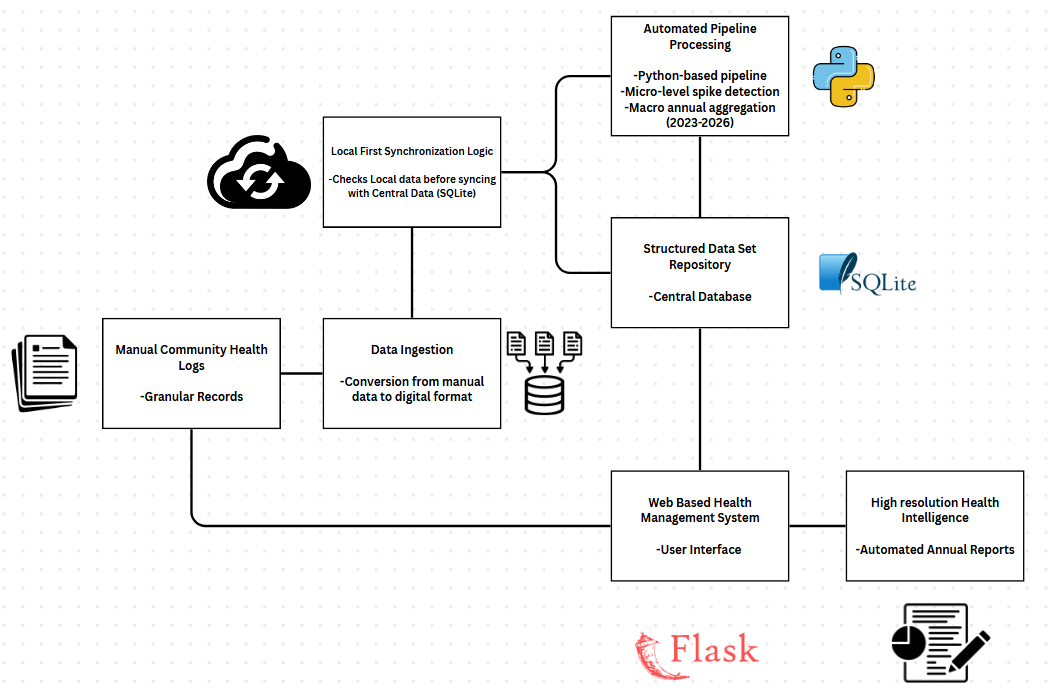
\includegraphics[width=7.16667in,height=4.90375in]{./media/image3.png}

\textbf{Figure 3.1. \emph{Conceptual Framework of the System.}}

\textbf{3.1.1 Input Stage}

The system initiates with the ingestion of manual community health logs,
which currently exist as granular, unstructured records. This stage
focuses on \textbf{Data Ingestion}, where manual entries are converted
into a digital format suitable for computational processing.

\textbf{3.1.2 Process Stage}

The processing core utilizes a hybrid architecture to ensure data
integrity, resilience, and analytical depth:

\begin{itemize}
\item
  \textbf{Local-First Synchronization Logic:} This component employs a
  synchronization protocol that verifies local data states before
  merging offline entries with the central data repository.
\item
  \textbf{Automated Pipeline Processing:} A Python-based processing
  pipeline handles computational logic, performing both micro-level
  processing (e.g., localized daily spike detection per purok) and
  multi-year chronological aggregation (2023--2026) to generate
  structured annual summaries.
\item
  \textbf{Structured Dataset Repository:} A central SQLite database
  serves as the normalized repository for all verified and de-identified
  medical records
\end{itemize}

\textbf{3.1.3 Output Stage}

The system culminates in the \textbf{Web-Based Health Management
System}, which provides a user interface for data interaction. The
primary output is \textbf{High-resolution Health Intelligence},
specifically delivered through \textbf{Automated Annual Reports}
designed to assist stakeholders in disease surveillance and resource
allocation.

\textbf{3.2 Operational Framework}

The operational framework (see Figure 3.2) delineates the sequential
workflow and procedural stages required to execute the study. While the
conceptual framework defines the system's architecture, the operational
framework serves as a procedural roadmap, mapping the transition from
the collection of health record logs to the generation of validated
reports.

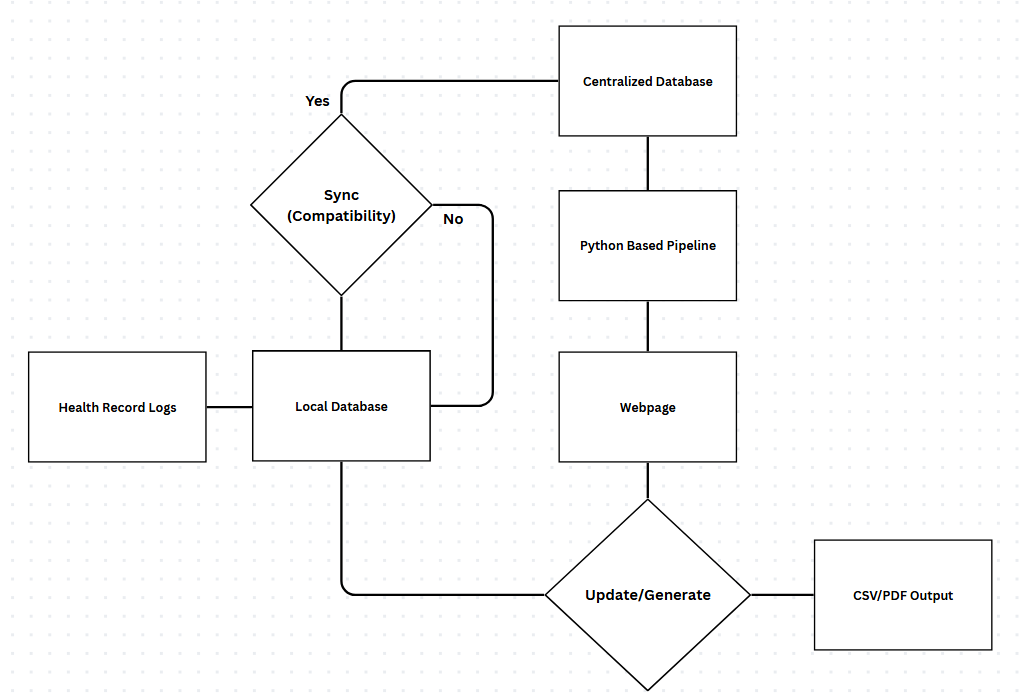
\includegraphics[width=7.14352in,height=3.98958in]{./media/image2.png}

\textbf{Figure 3.2. \emph{Operational Framework of the Study.}}

\textbf{3.2.1 Phase I: Data Acquisition and Local Storage}

The initial phase focuses on the ingestion and primary storage of health
records, transitioning manual paper logs into a digital pipeline.

\begin{itemize}
\item
  \textbf{Local Database Entry:} Data is captured locally in SQLite
  (lokalhealth.db), allowing Barangay Health Workers (BHWs) to record
  cases offline. Each entry stores six core schema parameters:
  consultation\_date, purok\_id, disease\_id, age, gender, and symptoms.
\item
  \textbf{De-Identification \& Anonymization Protocol:} To comply with
  the Data Privacy Act of 2012 (RA 10173), direct identifiers like names
  and contact details are excluded. Records receive auto-generated
  internal case keys (id) at entry to ensure full patient
  de-identification.
\end{itemize}

\textbf{3.2.2 Phase II: Synchronization and Compatibility Logic}

This phase manages data validation and integration across storage tiers.

\begin{itemize}
\item
  \textbf{Compatibility Check:} The system evaluates offline local logs
  to ensure structural compatibility and prevent duplicate entries
  before merging.
\item
  \textbf{Centralized Integration:} Verified logs are pushed to the
  central database repository for long-term storage and analytical
  processing. \textbackslash{}
\end{itemize}

\textbf{3.2.3 Phase III: Processing and Web Interface}

This phase transforms raw stored records into actionable health
analytics using a Python-based processing pipeline.

\begin{itemize}
\item
  \textbf{Seasonal Bias Control:} To balance monsoon/flood spikes
  (Dengue, Leptospirosis) against endemic baseline diseases (TB), the
  pipeline evaluates records across full 12-month cycles (2023--2026)
  using month-over-month rate comparisons.
\item
  \textbf{Geographical Bias Control:} Mapping records to purok\_id
  isolates spatial risk factors, distinguishing high-density urban zones
  from flood-prone riverbank areas.
\item
  \textbf{Chronological Partitioning:} To prevent temporal data leakage,
  historical records from 2023--2025 serve as the baseline analysis
  dataset, while 2026 records are partitioned as the evaluation test
  set.
\item
  \textbf{Web Interface Rendering:} Processed analytics are delivered to
  the web dashboard, providing interactive visualizations for BHWs and
  Administrators.
\end{itemize}

\textbf{3.2.4 Phase IV: Output and Reporting}

The final phase focuses on delivering structured epidemiological outputs
to municipal health authorities.

\begin{itemize}
\item
  \textbf{Dual-Level Visibility:} The reporting module provides granular
  case-level tracking for internal clinic operations and aggregated
  monthly/annual summaries for macro-surveillance.
\item
  \textbf{CSV/PDF Export Generation:} Standardized summary reports are
  rendered into downloadable CSV and PDF formats for seamless submission
  to the City Health Office (CHO).
\end{itemize}

\subsubsection{\texorpdfstring{\textbf{References}}{References}}\label{references}

J. Alderden, P. D. Sharkey, S. M. Kennerly, S. Ghosh, R. S. Barrett, S.
D. Horn, S. Ghosh, and T. L. Yap. 2023. Developing a relational database
for best practice data management: The TEAM-UP database. Computers,
Informatics,
Nursing.\href{https://pmc.ncbi.nlm.nih.gov/articles/PMC10153087/}{\ul{https://pmc.ncbi.nlm.nih.gov/articles/PMC10153087/}}

J. Antas, R. R. Silva, and J. Bernardino. 2022. Assessment of SQL and
NoSQL systems to store and mine COVID-19 data. \emph{Computers}.
\href{https://www.mdpi.com/2073-431X/11/2/29}{\ul{https://www.mdpi.com/2073-431X/11/2/29}}

R. E. Baticulon, J. J. Sy, N. R. Alberto, M. B. C. Baron, R. E. C.
Mabulay, L. G. T. Rizada, C. J. S. Tiu, C. A. Clarion, J. C. B. Reyes,
et al. 2021. Barriers to online learning in the time of COVID-19: A
national survey of medical students in the Philippines. \emph{Medical
Science Educator}.
\href{https://link.springer.com/article/10.1007/s40670-021-01231-z}{\ul{https://link.springer.com/article/10.1007/s40670-021-01231-z}}

Z. Chengyu, H. Xueyan, and F. Ying. 2024. Research on disease management
of chronic disease patients based on digital therapeutics: A scoping
review. \emph{Journal of Medical Internet Research}.
\href{https://pmc.ncbi.nlm.nih.gov/articles/PMC11544657/}{\ul{https://pmc.ncbi.nlm.nih.gov/articles/PMC11544657/}}

R. Y. H. De Mesa, Z. M. Hendrickson, C. S. C. Tan-Lim, A. Elepaño, N. M.
C. Fabian, J. F. E. Lopez, C. A. Latkin, L. F. Dans, M. P. Rey, and A.
M. L. Dans. 2023. Resilience, ingenuity, and identity: A multi-level
analysis of the Filipino community health worker experience in rural and
remote municipalities in the Philippines. \emph{PLOS Global Public
Health}.
\href{https://doi.org/10.1371/journal.pgph.0004965}{\ul{https://doi.org/10.1371/journal.pgph.0004965}}

M. Glennie, M. Dowden, M. Scolyer, I. O'Meara, G. Angeles, H. Woerle, P.
T. Campbell, and K. Gardner. 2023. Community-led data collection:
Enhancing local-level scabies surveillance in remote Aboriginal
communities in Australia. \emph{Tropical Medicine and Infectious
Disease}.
\href{https://www.mdpi.com/2414-6366/8/4/200}{\ul{https://www.mdpi.com/2414-6366/8/4/200}}

K. Y. Hartigan-Go, M. L. Prieto, and S. A. Valenzuela. 2024. Important
but neglected: A qualitative study on the lived experiences of barangay
health workers in the Philippines. \emph{Acta Medica Philippina}.
\href{https://actamedicaphilippina.upm.edu.ph/index.php/acta/article/view/9589}{\ul{https://actamedicaphilippina.upm.edu.ph/index.php/acta/article/view/9589}}

I. Izonin, R. Tkachenko, N. Shakhovska, B. Ilchyshyn, and K. K. Singh.
2022. A two-step data normalization approach for improving
classification accuracy in the medical diagnosis domain.
\emph{Mathematics}.
\href{https://www.mdpi.com/2227-7390/10/11/1942}{\ul{https://www.mdpi.com/2227-7390/10/11/1942}}

S. S. Jazaeri, P. Asghari, S. Jabbehdari, and H. H. S. Javadi. 2023.
Composition of caching and classification in edge computing based on
quality optimization for SDN-based IoT healthcare solutions.
\emph{Sensors}.
\href{https://pmc.ncbi.nlm.nih.gov/articles/PMC10169185/}{\ul{https://pmc.ncbi.nlm.nih.gov/articles/PMC10169185/}}

S. S. Kaboré, P. Ngangue, D. Soubeiga, A. Barro, A. H. Pilabré, N.
Bationo, Y. Pafadnam, K. M. Drabo, H. Hien, and G. B. L. Savadogo. 2022.
Barriers and facilitators for the sustainability of digital health
interventions in low- and middle-income countries: A systematic review.
\emph{BMC Health Services Research}.
\href{https://pmc.ncbi.nlm.nih.gov/articles/PMC9742266/}{\ul{https://pmc.ncbi.nlm.nih.gov/articles/PMC9742266/}}

P. K. Krishnapur, C. Cm, A. B, and A. M. 2026. A reproducible
Python-based computational pipeline for real-time ingestion, advanced
analysis, and dynamic reporting of public health data: A systems
validation study. \emph{Journal of Medical Internet Research}.
\href{https://pubmed.ncbi.nlm.nih.gov/41798472/}{\ul{https://pubmed.ncbi.nlm.nih.gov/41798472/}}

J. Li, X. Luo, and H. Lei. 2024. TrustHealth: Enhancing eHealth Security
with Blockchain and Trusted Execution Environments. \emph{Electronics}.
\href{https://www.mdpi.com/2079-9292/13/12/2425}{\ul{https://www.mdpi.com/2079-9292/13/12/2425}}

S. Li, K. Peng, B. Zhu, Z. Li, B. Zhang, H. Chen, and R. Li. 2023.
Research on Users' Privacy-Sharing Intentions in the Health Data
Tracking System Providing Personalized Services and Public Services.
\emph{Sustainability}.
\href{https://www.mdpi.com/2071-1050/15/22/15709}{\ul{https://www.mdpi.com/2071-1050/15/22/15709}}

B. Negreiros, S. Schwindt, F. Scolari, R. Barros, A. A. Galdos, M.
Noack, S. Haun, and S. Wieprecht. 2024. A database application framework
toward data-driven vertical connectivity analysis of rivers.
\emph{Environmental Modelling \& Software}.
\href{https://www.sciencedirect.com/science/article/pii/S136481522300302X}{\ul{https://www.sciencedirect.com/science/article/pii/S136481522300302X}}

H. S. Ngusie, A. M. Shiferaw, A. D. Bogale, and M. H. Ahmed. 2021.
Health data management practice and associated factors among health
professionals working at public health facilities in resource-limited
settings. \emph{BMC Medical Informatics and Decision Making}.
\href{https://pmc.ncbi.nlm.nih.gov/articles/PMC8357531/}{\ul{https://pmc.ncbi.nlm.nih.gov/articles/PMC8357531/}}

J. A. Obiri-Tetteh, R. E. Turkson, E. A. Frimpong, A. S. Yussif, D. A.
Asante, and E. Attipoe. 2021. BCrypt-Based Optimized Password Hashing
Against Targeted Internet of Things Attacks. \emph{Cureus}.
\href{https://www.cureusjournals.com/articles/5167-bcrypt-based-optimized-password-hashing-against-targeted-internet-of-things-attacks\#!/}{\ul{https://www.cureusjournals.com/articles/5167-bcrypt-based-optimized-password-hashing-against-targeted-internet-of-things-attacks\#!/}}

R. S. Oktaviana, P. W. Handayani, A. N. Hidayanto, and B. B. Siswanto.
2025. Healthcare data governance assessment based on hospital management
perspectives. \emph{International Journal of Information Management Data
Insights}.
\href{https://www.sciencedirect.com/science/article/pii/S2667096825000242}{\ul{https://www.sciencedirect.com/science/article/pii/S2667096825000242}}

M. C. B. Otero, L. A. E. Murao, M. A. G. Limen, D. R. A. Caalim, P. L.
A. Gaite, M. G. Bacus, J. T. Acaso, R. M. Miguel, K. Corazo, I. E. Knot,
et al. 2022. Multifaceted assessment of wastewater-based epidemiology
for SARS-CoV-2 in selected urban communities in Davao City, Philippines:
A pilot study. \emph{Science of the Total Environment}.
\href{https://pmc.ncbi.nlm.nih.gov/articles/PMC9324557/}{\ul{https://pmc.ncbi.nlm.nih.gov/articles/PMC9324557/}}

J. Paluyo, A. Stake, and R. Bryson. 2022. ``Padayon'': A new digital
health model for diabetes and hypertension in rural Philippines.
\emph{BMJ Innovations}.
\href{https://innovations.bmj.com/content/9/1/43}{\ul{https://innovations.bmj.com/content/9/1/43}}

K. Rahul and R. K. Banyal. 2020. Data life cycle management in big data
analytics. \emph{Procedia Computer Science}.
\href{https://www.sciencedirect.com/science/article/pii/S1877050920315465}{\ul{https://www.sciencedirect.com/science/article/pii/S1877050920315465}}

N. Spiridonova, E. Andrianova, E. Rezedinova, and A. Schukin. 2025.
Developing a portal for learning relational databases with automatic SQL
validation. \emph{Computer Science and Information Systems}.
\href{https://www.mdpi.com/2673-4591/104/1/89}{\ul{https://www.mdpi.com/2673-4591/104/1/89}}

P. G. Sylim, J. L. Lu, and P. G. F. Marcelo. 2022. Discoursing
terminology standards and interoperability in relation to the Philippine
eHealth strategy. \emph{Acta Medica Philippina}.
\href{https://actamedicaphilippina.upm.edu.ph/index.php/acta/article/view/3937}{\ul{https://actamedicaphilippina.upm.edu.ph/index.php/acta/article/view/3937}}

A. Thakur, R. Bhageerathy, P. Mithra, V. Chandra Sekaran, and S. Kumar.
2023. Navigating organizational challenges of digital transformation: A
qualitative study of meso-level public health officers in an Indian
high-priority aspirational district. \emph{International Journal of
Medical Informatics}.
\href{https://www.mdpi.com/2076-3387/15/10/397}{\ul{https://www.mdpi.com/2076-3387/15/10/397}}

D. Trillo-Montero, S. Cosano-Lucena, M. González-Redondo, J. J.
Luna-Rodríguez, and I. Santiago. 2023. Design and development of a
relational database management system (RDBMS) with open-source tools for
the processing of data monitored in a set of photovoltaic (PV) plants.
\emph{Applied Sciences}.
\href{https://www.mdpi.com/2076-3417/13/3/1357}{\ul{https://www.mdpi.com/2076-3417/13/3/1357}}

L. Whitehead, J. Talevski, F. Fatehi, and A. Beauchamp. 2023. Barriers
to and facilitators of digital health among culturally and
linguistically diverse populations: A qualitative systematic review.
\emph{International Journal of Medical Informatics}.
\href{https://www.sciencedirect.com/org/science/article/pii/S1438887123001085}{\ul{https://www.sciencedirect.com/org/science/article/pii/S1438887123001085}}

\end{document}
